\section{Alit Fajar Kurniawan 1174057}
\subsection{Pemahaman Teori}
	\begin{enumerate}

		\item Apa itu fungsi library matplotlib ?
			\subitem Matplotlib adalah suatu library Python 2D yang dapat menghasilkan plot dengan kualitas yang tinggi dalam berbagai format dan dapat digunakan di berbagai platform. Matplotlib berfungsi sebagai pembuat grafik di berbagai platform, seperti Python dan Jupyter. Grafik yang dibuat menggunakan Matplotlib bisa dibuat dalam berbagai bentuk, seperti grafik garis, batang, lingkaran, histogram, dan sebagainya.
		
		\item Jelaskan langkah-langkah membuat sumbu X dan Y di matplotlib
			\begin{itemize}
				\item Pertama import library Matplotlib.	
				\lstinputlisting[firstline=2, lastline=2]{src/chapter6/1174057/1174057.py}
				
				\item Buat variabel x yang menampung list untuk sumbu x dan variabel y yang menampung list untuk sumbu y.	
				\lstinputlisting[firstline=4, lastline=5]{src/chapter6/1174057/1174057.py}
				
				\item Panggil fungsi plot dan isi parameter pertama dengan variabel x dan parameter kedua dengan variabel y.
				\lstinputlisting[firstline=7, lastline=7]{src/chapter6/1174057/1174057.py}	

				\item Lalu panggil plot tadi dengan memanggil fungsi show.
				\lstinputlisting[firstline=9, lastline=9]{src/chapter6/1174057/1174057.py}
			\end{itemize}

			\hfill \break
			\textbf{Kode Program}
			
				\lstinputlisting[caption = Kode program membuat diagram menggunakan Matplotlib., firstline=2, lastline=9]{src/chapter6/1174057/1174057.py}
				
			\hfill \break
			\textbf{Hasil Compile}

			\begin{figure}[H]
				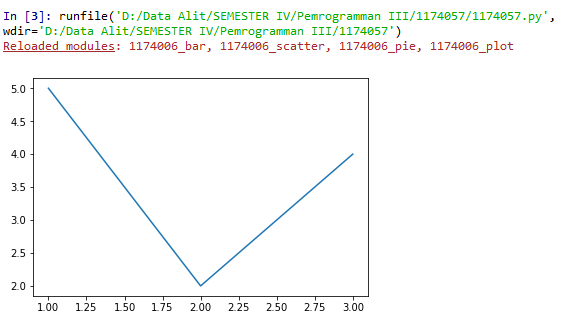
\includegraphics[width=12cm]{figures/chapter6/1174057/2.png}
				\centering
				\caption{Hasil compile membuat diagram menggunakan Matplotlib.}
			\end{figure}
			
		
		\item Jelaskan bagaimana perbedaan fungsi dan cara pakai untuk berbagai jesnis (bar, histogram, scatter, dll) jenis plot di matplotlib !
			\begin{itemize}
				\item \textbf{Bar Graph}
				
				Perbedaan bar graph dengan jenis plot yang lain adalah bar graph menggunakan bar atau batang-batang untuk membandingkan data di antara berbagai kategori.
				
				\textbf{Kode Program}
				
				\lstinputlisting[caption = Kode program membuat bar graph menggunakan Matplotlib., firstline=13, lastline=25]{src/chapter6/1174057/1174057.py}
				
				\textbf{Hasil Compile}
				
				\begin{figure}[H]
					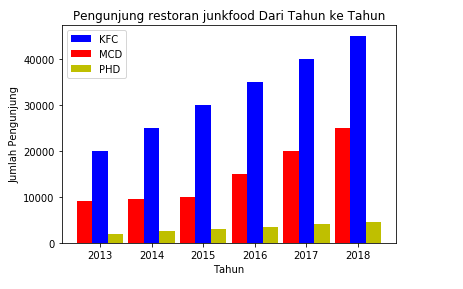
\includegraphics[width=12cm]{figures/chapter6/1174057/3.png}
					\centering
					\caption{Hasil compile membuat bar graph menggunakan Matplotlib.}
				\end{figure}
				
				\item \textbf{Histogram}
				
				Perbedaan histogram dengan jenis plot yang lain adalah histogram akan membuat plot dimana plot yang dimunculkan merupakan gabungan dari beberapa data yang telah dikelompokkan.
				
				\textbf{Kode Program}
				
				\lstinputlisting[caption = Kode program membuat histogram menggunakan Matplotlib., firstline=29, lastline=36]{src/chapter6/1174057/1174057.py}
				
				\textbf{Hasil Compile}
				
				\begin{figure}[H]
					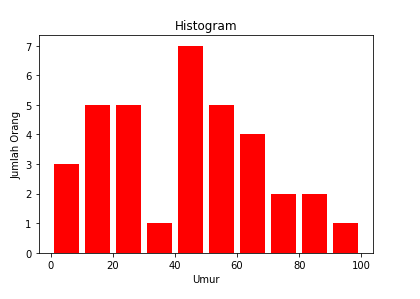
\includegraphics[width=12cm]{figures/chapter6/1174057/3histogram.png}
					\centering
					\caption{Hasil compile membuat histogram menggunakan Matplotlib.}
				\end{figure}
				
				\item \textbf{Scatter Plot}
				
				Perbedaan scatter plot dengan jenis plot lain adalah scatter plot menampilkan data sebagai kumpulan titik, masing-masing memiliki nilai satu variabel yang menentukan posisi pada sumbu horizontal dan nilai variabel lain menentukan posisi pada sumbu vertikal.
				
				\textbf{Kode Program}
				
				\lstinputlisting[caption = Kode program membuat scatter plot menggunakan Matplotlib., firstline=40, lastline=53]{src/chapter6/1174057/1174057.py}
				
				\textbf{Hasil Compile}
				
				\begin{figure}[H]
					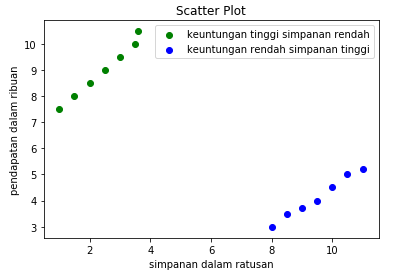
\includegraphics[width=12cm]{figures/chapter6/1174057/3scatter.png}
					\centering
					\caption{Hasil compile membuat scatter plot menggunakan Matplotlib.}
				\end{figure}
				
				\item \textbf{Area Plot}
				
				Perbedaan area plot dengan jenis plot lain adalah area plot digunakan untuk melacak perubahan dari waktu ke waktu untuk dua atau lebih kelompok terkait yang membentuk satu kategori secara keseluruhan.
				
				\textbf{Kode Program}
				
				\lstinputlisting[caption = Kode program membuat diagram menggunakan Matplotlib., firstline=57, lastline=76]{src/chapter6/1174057/1174057.py}
				
				\textbf{Hasil Compile}
				
				\begin{figure}[H]
					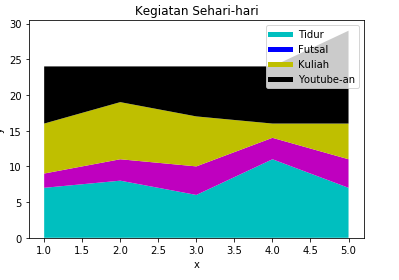
\includegraphics[width=12cm]{figures/chapter6/1174057/3area.png}
					\centering
					\caption{Hasil compile membuat diagram menggunakan Matplotlib.}
				\end{figure}
				
				\item \textbf{Pie Plot}
				
				Perbedaan pie plot dengan jenis plot lain adalah pie plot digunakan untuk menunjukkan persentase atau data proporsional di mana setiap potongan pie mewakili kategori.
				
				\textbf{Kode Program}
				
				\lstinputlisting[caption = Kode program membuat Pie Plot menggunakan Matplotlib., firstline=86, lastline=101]{src/chapter6/1174057/1174057.py}
				
				\textbf{Hasil Compile}
				
				\begin{figure}[H]
					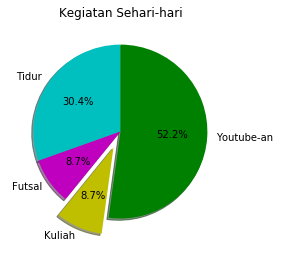
\includegraphics[width=9cm]{figures/chapter6/1174057/3pie.png}
					\centering
					\caption{Hasil compile membuat Pie Plot menggunakan Matplotlib.}
				\end{figure}
				
				\item \textbf{Line Graph}
				
				Perbedaan line graph dengan jenis plot lain adalah line graph menampilkan diagram dalam bentuk garis.
				
				\textbf{Kode Program}
				
				\lstinputlisting[caption = Kode program membuat diagram menggunakan Matplotlib., firstline=105, lastline=113]{src/chapter6/1174057/1174057.py}
				
				\textbf{Hasil Compile}
				
				\begin{figure}[H]
					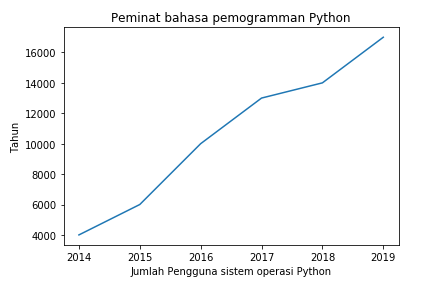
\includegraphics[width=12cm]{figures/chapter6/1174057/3line.png}
					\centering
					\caption{Hasil compile membuat diagram menggunakan Matplotlib.}
				\end{figure}
				
			\end{itemize}
		
		\item Jelaskan bagaimana cara menggunakan legend dan label serta kaitannya fungsi tersebut !
			\begin{itemize}
				\item Untuk menggunakan legend definisikan parameter label di tiap fungsi plot. Parameter label digunakan untuk memberikan label pada line sebagai pembeda antar line.
				
				\lstinputlisting[caption = Kode program menggunakan parameter label dengan Matplotlib., firstline=123, lastline=124]{src/chapter6/1174057/1174057.py}
				
				\item Kemudian panggil fungsi legend.
				
				\lstinputlisting[caption = Kode program memanggil fungsi legend dengan Matplotlib., firstline=128, lastline=128]{src/chapter6/1174057/1174057.py}
			\end{itemize}

			\hfill \break
			\textbf{Kode Program}

			\lstinputlisting[caption = Kode program membuat diagram menggunakan Matplotlib., firstline=117, lastline=130]{src/chapter6/1174057/1174057.py}

			\hfill \break
			\textbf{Hasil Compile}

			\begin{figure}[H]
				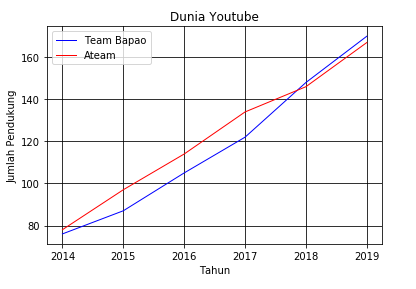
\includegraphics[width=12cm]{figures/chapter6/1174057/4.png}
				\centering
				\caption{Hasil compile membuat diagram menggunakan Matplotlib.}
			\end{figure}
	
		\item Jelaskan apa fungsi dari subplot di matplotlib, dan bagaimana cara kerja dari fungsi subplot, sertakan ilustrasi dan gambar sendiri dan apa parameternya jika ingin menggambar plot dengan 9 subplot di dalamnya!
			\hfill \break
			Fungsi subplot adalah untuk membuat beberapa plot di dalam satu gambar.
			\hfill \break
			Cara kerja subplot, yaitu fungsi subplot memiliki parameter pertama adalah jumlah kolom, parameter kedua adalah jumlah baris, dan parameter ketiga adalah index plot keberapanya.

			\hfill \break
			\textbf{Kode Program}

			\lstinputlisting[caption = Kode program membuat subplot menggunakan Matplotlib., firstline=134, lastline=146]{src/chapter6/1174057/1174057.py}

			\hfill \break
			\textbf{Hasil Compile}

			\begin{figure}[H]
				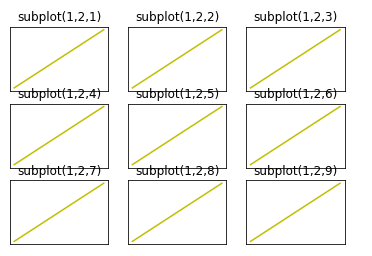
\includegraphics[width=12cm]{figures/chapter6/1174057/5subplot.png}
				\centering
				\caption{Hasil compile membuat subplot menggunakan Matplotlib.}
			\end{figure}

		\item Sebutkan semua parameter color yang bisa digunakan (contoh:  m,c,r,k,...  dkk)!
		
			\begin{itemize}
				\item 'b' (blue)
				\item 'g' (green)
				\item 'r' (red)
				\item 'c' (cyan)
				\item 'm' (magenta)
				\item 'y' (yellow)
				\item 'k' (black)
				\item 'w' (white)
			\end{itemize}

		\item Jelaskan bagaimana cara kerja dari fungsi hist, sertakan ilustrasi dan gambar sendiri!

			\hfill \break
			Cara kerja dari fungsi hist yaitu fungsi hist akan menerima parameter yang diberikan, kemudian fungsi hist akan dieksekusi sesuai dengan parameter yang diberikan.

			\hfill \break
			\textbf{Kode Program}

			\lstinputlisting[caption = Kode program membuat diagram menggunakan Matplotlib., firstline=150, lastline=157]{src/chapter6/1174057/1174057.py}

			\hfill \break
			\textbf{Hasil Compile}

			\begin{figure}[H]
				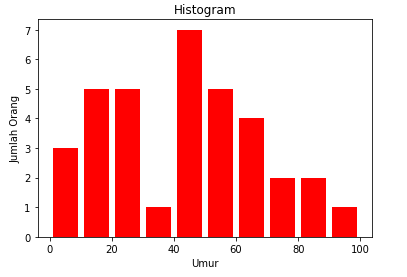
\includegraphics[width=12cm]{figures/chapter6/1174057/7histogram.png}
				\centering
				\caption{Hasil compile membuat diagram menggunakan Matplotlib.}
			\end{figure}
			
		\item Jelaskan lebih mendalam tentang parameter dari fungsi pie diantaranya labels, colors, startangle, shadow, explode, autopct!
 
			 \begin{itemize}
				\item labels : untuk memberikan label di tiap persentase.
				\item colors : untuk memberikan warna di tiap persentase.
				\item startangle : untuk memutar plot sesuai dengan derajat yang ditentukan.
				\item shadow : untuk memberikan bayangan pada plot.
				\item explode : untuk memisahkan antar tiap potongan pie pada plot.
				\item autopct : untuk menentukan jumlah angka dibelakang koma.
			 \end{itemize}
		
	\end{enumerate}
	
	\subsection{Keterampilan Pemogramman}
	\begin{enumerate}
		\item Buatlah librari fungsi (file terpisah/library dengan nama NPMbar.py) untuk plot dengan jumlah subplot adalah NPM mod 3 + 2!

			\hfill \break
			\textbf{Kode Program}

			\lstinputlisting[caption = Kode program membuat fungsi Bar Plot menggunakan Matplotlib., firstline=1, lastline=21]{src/chapter6/1174057/1174057_bar.py}

			\hfill \break
			\textbf{Hasil Compile}

			\begin{figure}[H]
				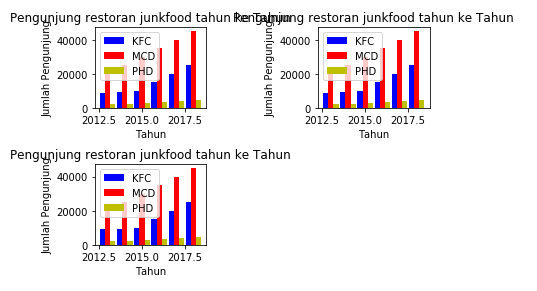
\includegraphics[width=12cm]{figures/chapter6/1174057/praktek1.png}
				\centering
				\caption{Hasil compile membuat fungsi Bar Plot menggunakan Matplotlib.}
			\end{figure}
			
		\item Buatlah librari fungsi (file terpisah/library dengan nama NPMscatter.py) untuk plot dengan jumlah subplot NPM mod 3 + 2!
					
			\hfill \break
			\textbf{Kode Program}

			\lstinputlisting[caption = Kode program membuat fungsi Scatter Plot menggunakan Matplotlib., firstline=1, lastline=23]{src/chapter6/1174057/1174057_scatter.py}

			\hfill \break
			\textbf{Hasil Compile}

			\begin{figure}[H]
				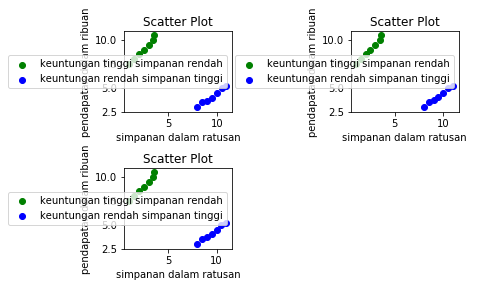
\includegraphics[width=12cm]{figures/chapter6/1174057/praktek2.png}
				\centering
				\caption{Hasil compile membuat fungsi Scatter Plot menggunakan Matplotlib.}
			\end{figure}

		\item Buatlah librari fungsi (file terpisah/library dengan nama NPMpie.py) untuk plot dengan jumlah subplot NPM mod 3 + 2!

			\hfill \break
			\textbf{Kode Program}

			\lstinputlisting[caption = Kode program membuat fungsi Pie Plot menggunakan Matplotlib., firstline=1, lastline=23]{src/chapter6/1174057/1174057_pie.py}

			\hfill \break
			\textbf{Hasil Compile}

			\begin{figure}[H]
				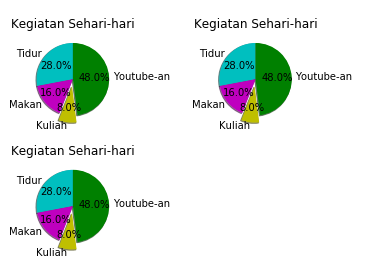
\includegraphics[width=12cm]{figures/chapter6/1174057/praktek3.png}
				\centering
				\caption{Hasil compile membuat fungsi Pie Plot menggunakan Matplotlib.}
			\end{figure}
			
		\item Buatlah librari fungsi (file terpisah/library dengan nama NPMplot.py) untuk plot dengan jumlah subplot NPM mod 3 + 2

			\hfill \break
			\textbf{Kode Program}

			\lstinputlisting[caption = Kode program membuat fungsi Plot menggunakan Matplotlib., firstline=1, lastline=23]{src/chapter6/1174057/1174057_plot.py}

			\hfill \break
			\textbf{Hasil Compile}

			\begin{figure}[H]
				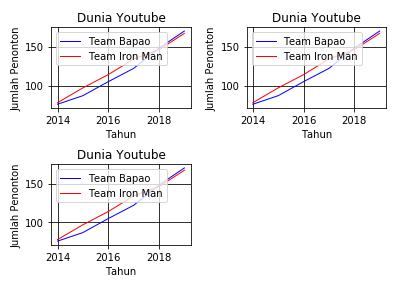
\includegraphics[width=12cm]{figures/chapter6/1174057/praktek4.png}
				\centering
				\caption{Hasil compile membuat fungsi Plot menggunakan Matplotlib.}
			\end{figure}	
	\end{enumerate}
	
	\subsection{Keterampilan Penanganan Error}
		Tuliskan  peringatan  error  yang  didapat  dari  mengerjakan  praktek  keenam  ini, dan  jelaskan  cara  penanganan  error  tersebut. dan  Buatlah  satu  fungsi  yang menggunakan try except untuk menanggulangi error tersebut.

		\hfill \break
		Peringatan error di praktek kelima ini, yaitu:
		\begin{itemize}
			\item Syntax Errors
			Syntax Errors adalah suatu keadaan saat kode python mengalami kesalahan penulisan. Solusinya adalah memperbaiki penulisan kode yang salah.
			
			\item Name Error
			NameError adalah exception yang terjadi saat kode melakukan eksekusi terhadap local name atau global name yang tidak terdefinisi. Solusinya adalah memastikan variabel atau function yang dipanggil ada atau tidak salah ketik.
			
			\item Type Error
			TypeError adalah exception yang akan terjadi apabila pada saat dilakukannya eksekusi terhadap suatu operasi atau fungsi dengan type object yang tidak sesuai. Solusi dari error ini adalah mengkoversi varibelnya sesuai dengan tipe data yang akan digunakan.
		\end{itemize}
		\hfill \break
		Fungsi yang menggunakan try except untuk menanggulangi error.

		\hfill \break
		\textbf{Kode Program}

		\lstinputlisting[caption = Kode program membuat fungsi penanganan error., firstline=161, lastline=178]{src/chapter6/1174057/1174057.py}

		\hfill \break
		\textbf{Hasil Compile}

		\begin{figure}[H]
			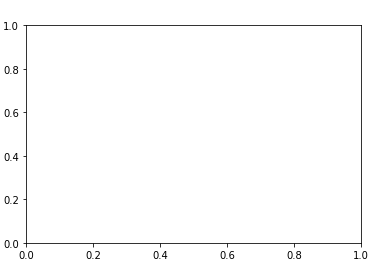
\includegraphics[width=12cm]{figures/chapter6/1174057/error.png}
			\centering
			\caption{hasil run penanganan error}
		\end{figure}
		
		\subsection{Screenshoot Plagiat}
		\begin{figure}[H]
			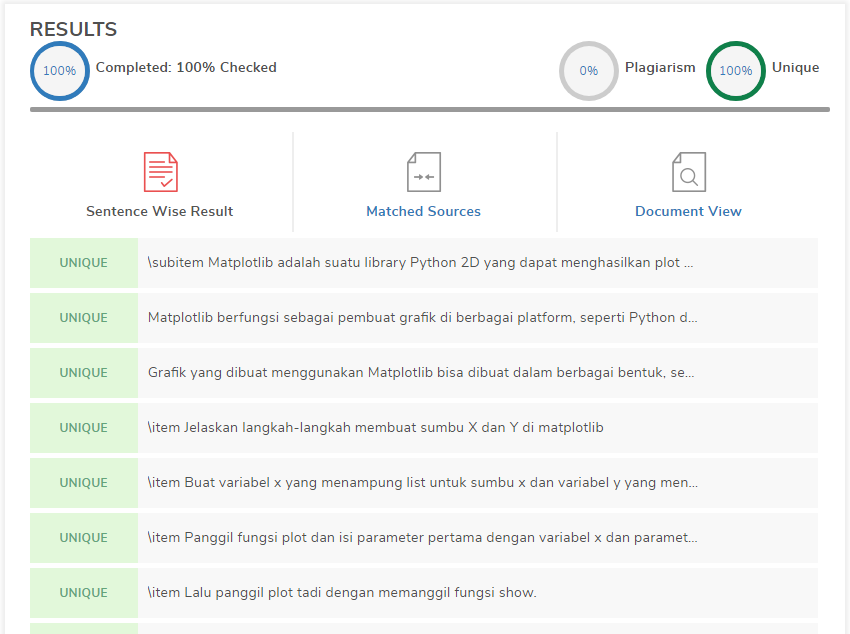
\includegraphics[width=12cm]{figures/chapter6/1174057/plagiarisme.png}
			\centering
		\end{figure}
		
		\subsection{Screenshoot Kode Program}
		
		\begin{figure}[H]
			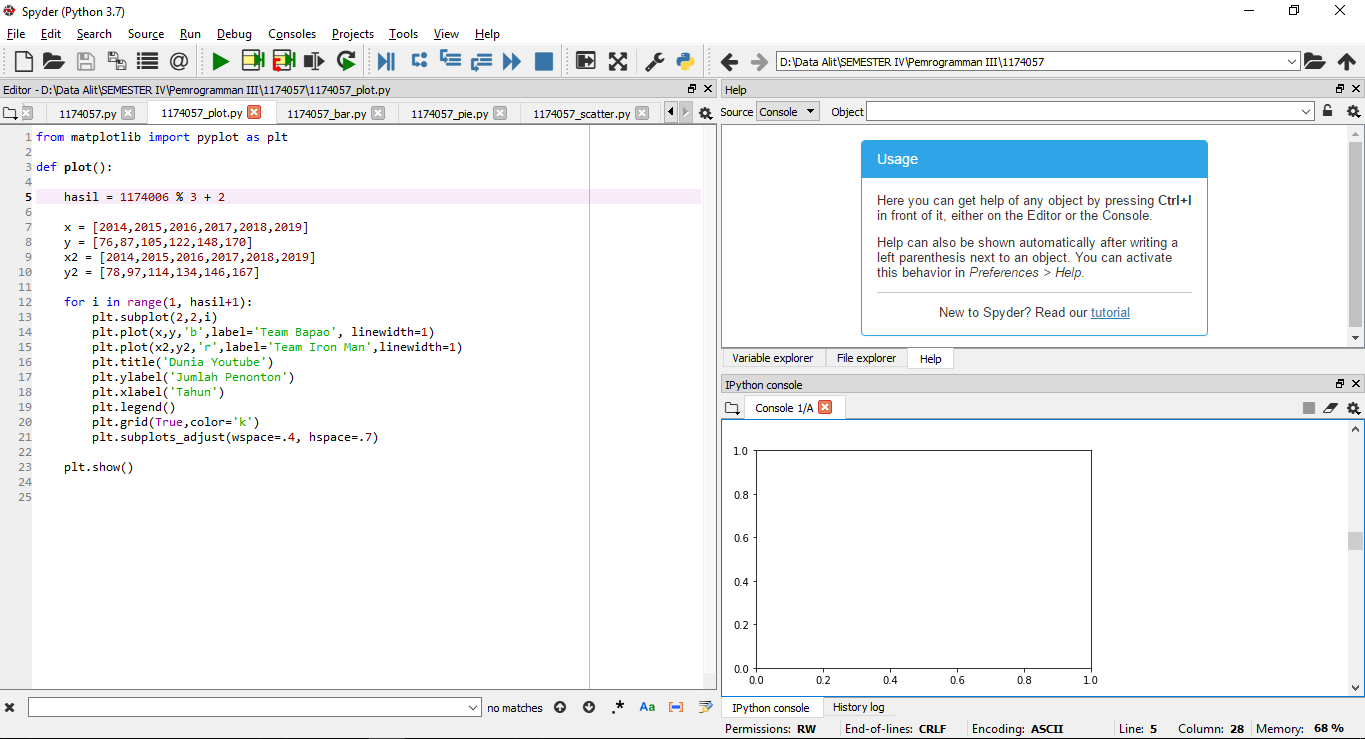
\includegraphics[width=9cm]{figures/chapter6/1174057/error1.png}
			\centering
			\centering
			\caption{hasil run penanganan error plot}
		\end{figure}
		\begin{figure}[H]
			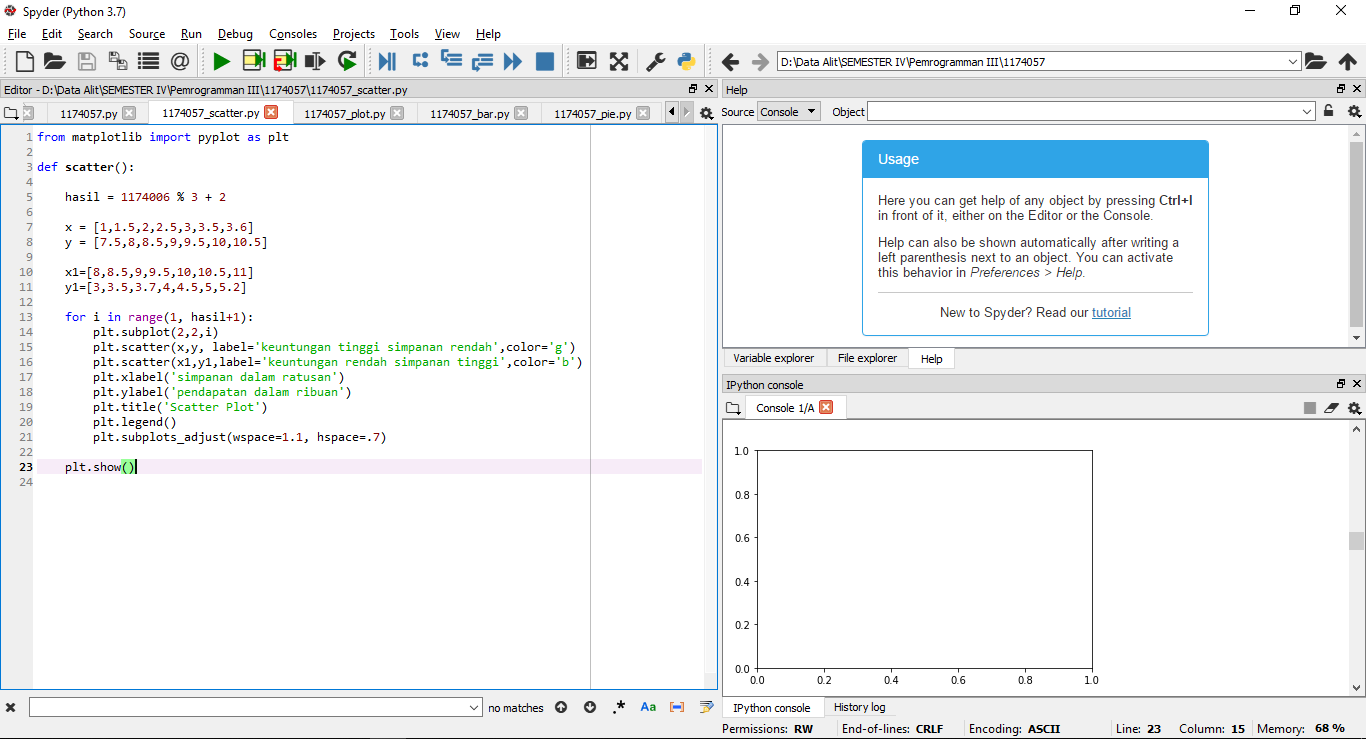
\includegraphics[width=9cm]{figures/chapter6/1174057/error2.png}
			\centering
			\centering
			\caption{hasil run penanganan error scatter}
		\end{figure}
		\begin{figure}[H]
			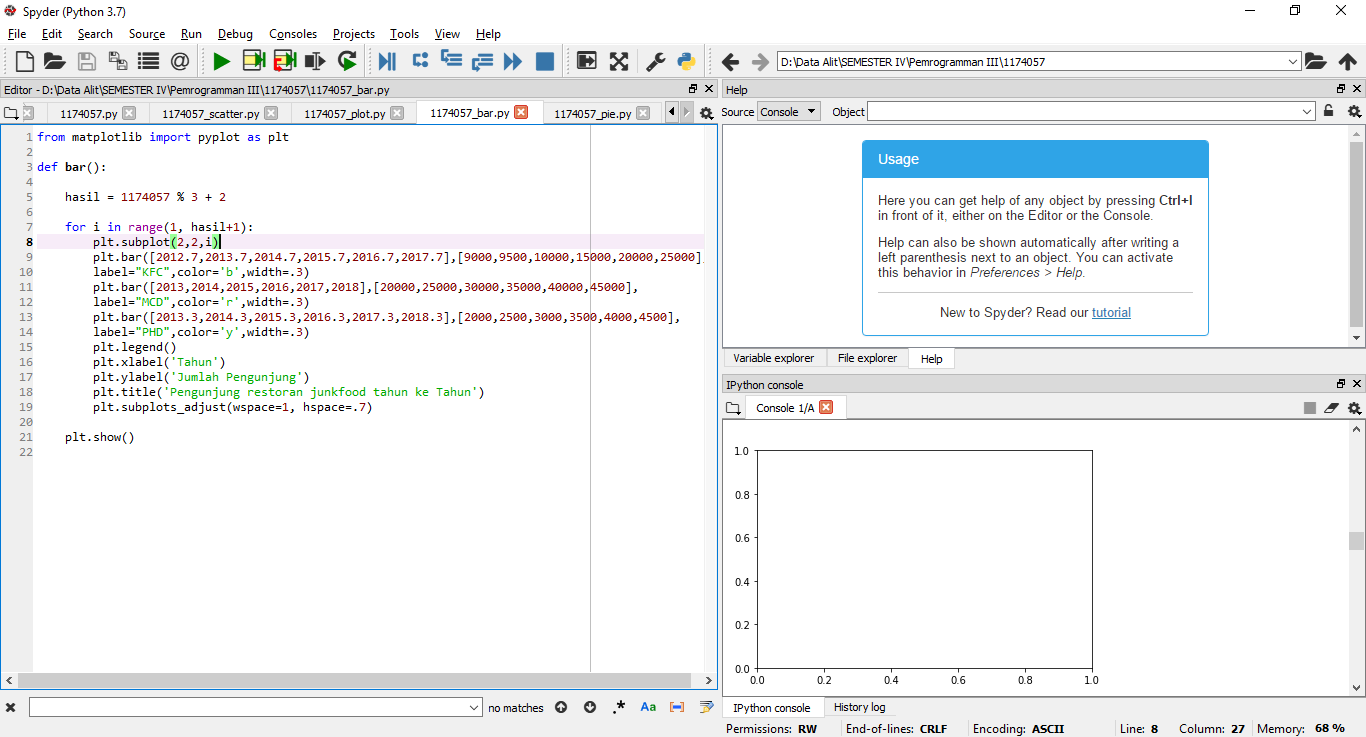
\includegraphics[width=9cm]{figures/chapter6/1174057/error3.png}
			\centering
			\centering
			\caption{hasil run penanganan error bar}
		\end{figure}
		\begin{figure}[H]
			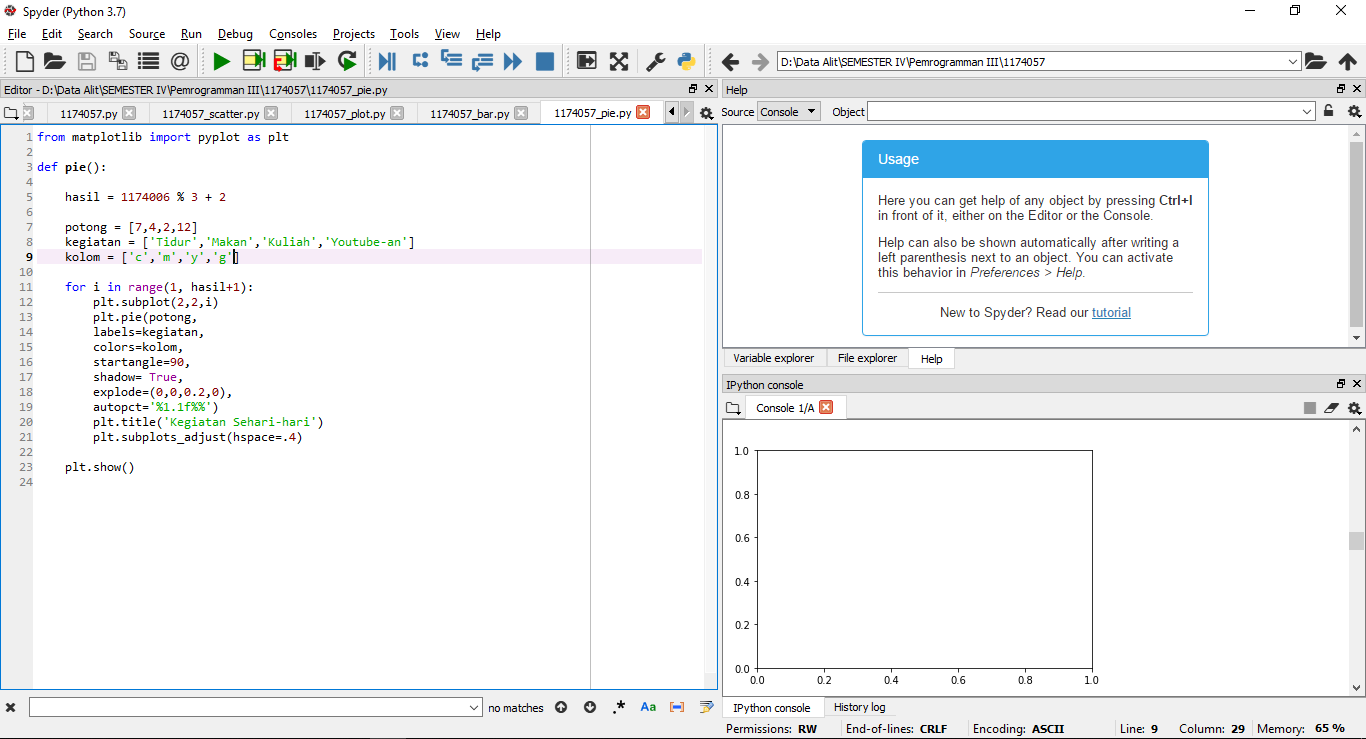
\includegraphics[width=9cm]{figures/chapter6/1174057/error4.png}
			\centering
			\centering
			\caption{hasil run penanganan error pie}
		\end{figure}
		
\section{Fathi Rabbani / 1164074}
\subsection{Teori}
\begin{enumerate}
\item Matplotlib
\par Library yang ada pada pemrograman Python yang berguna untuk membuat data grafik yang berdimensi 2.

\item Membuat Sumbu X dan Y
\par membuat sumbu X dan Y pada penggunaan Library Matplotlib adalah dengan menjelaskan setiap detail data array yang dimiliki sebagai contohnya ada pada Code Berikut : 
\lstinputlisting[firstline=3, lastline=8]{src/chapter6/1164074/code.py}

\item Penggunaan Jenis Plot di Matplotlib
\par ada berbagai macam Jenis PLot yang ada pada Matplotlib, diantaranya adalah :
\begin{itemize}
\item \lstinputlisting[firstline=2, lastline=8, caption=Jenis Garis]{src/chapter6/1164074/code.py}
\item \lstinputlisting[firstline=11, lastline=13, caption=Jenis Titik]{src/chapter6/1164074/code.py}
\item \lstinputlisting[firstline=16, lastline=20, caption=Jenis Batang]{src/chapter6/1164074/code.py}
\item \lstinputlisting[firstline=23, lastline=33, caption=Jenis Pie]{src/chapter6/1164074/code.py}
\end{itemize}

\item Menggunakan Legend dan Label
\par Legend pada matplotlib digunakan untuk menunjukan penggunaan grafik yang ditampilkan. contohnya dapat dilihat pada code berikut : 
\lstinputlisting[firstline=36, lastline=38, caption=Code penggunaan Legend pada Matplotlib]{src/chapter6/1164074/code.py}

\par Label pada matplotlib digunakan untuk menambahkan data Text pada grafik agar mudah untuk dibaca.
\lstinputlisting[firstline=42, lastline=45, caption=Code penggunaan Label pada Matplotlib]{src/chapter6/1164074/code.py}

\item Fungsi subplot di Matplotlib
\par Fungsi yang digunakan untuk menambahkan beberapa diagram sekaligus dalam satu sintaks. contoh code dan penggunaannya dapat dilihat pada Code dan Gambar \ref{data1}
\lstinputlisting[firstline=48, lastline=74, caption= Code penggunaan Subplot pada Matplotlib]{src/chapter6/1164074/code.py}
\begin{figure} [!htbp]
	\centerline{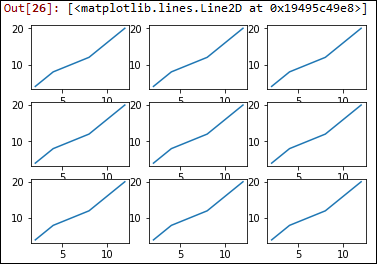
\includegraphics[width=0.5\textwidth]{figures/chapter6/1164074/1}}
	\caption{Penggunaan Subplot pada Matplotlib}
	\label{data1}
\end{figure}

\item Parameter Color
\par Penggunaan warna memiliki peran penting dalam membuat tampilan Grafik lebih menarik dan tidak membosankan, berikut ini adalah daftar penggunaan warna pada Matplotlib :

\begin{itemize}
	\item b : Untuk memberikan warna biru
	\item g : Untuk memberikan warna hijau
	\item r : Untuk memberikan warna merah
	\item c : Untuk memberikan warna biru muda
	\item m : Untuk memberikan warna pink
	\item y : Untuk memberikan warna kuning
	\item k : Untuk memberikan warna hitam
	\item w : Untuk memberikan warna putih
\end{itemize}


\item Cara kerja Fungsi hist
\par Fungsi Hist merupakan fungsi yang berguna untuk membuat data grafik Batang yang memiliki nilai banyak (Array). contoh Code dan penjelasanya dapat dilihat pada Gambar \ref{data2}
\lstinputlisting[firstline=77, lastline=81, caption= Code penggunaan Subplot pada Matplotlib]{src/chapter6/1164074/code.py}
\begin{figure} [!htbp]
	\centerline{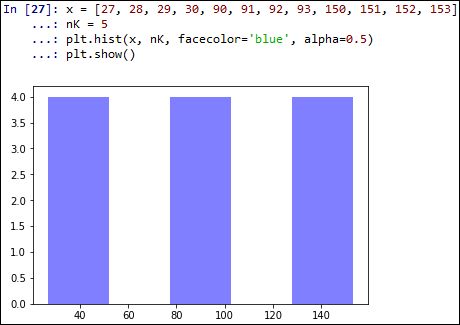
\includegraphics[width=0.5\textwidth]{figures/chapter6/1164074/2}}
	\caption{Hasil dari Penggunaan Hist dari Code tersebut}
	\label{data2}
\end{figure}

\item Keterangan Lebih tentang Parameter pada Fungsi Pie
\begin{itemize}
\item Labels
\par Isi dengan tipe data list dan tidak wajib untuk digunakan. Fungsi parameter labels untuk memberi label pada setiap pecahan data yang ada pada grafik pie yang ditampilkan.

\item Colors
\par Tipe data array atau sejenis dan tidak wajib untuk digunakan. Fungsi parameter colors untuk mengganti warna pada setiap pecahan yang ada. Jika tidak digunakan atau ditentukan, maka warna yang akan dipakai adalah warna yang aktif atau standar.
	
\item Startangle
\par Tipe data pecahan atau float, tidak wajib untuk digunakan. Fungsi parameter startangle adalah fungsi untuk memutar grafik agar berubah posisi dengan acuan yaitu angle awalan dari grafik pie.

	
\item Shadow
\par Bertipe data boolean dan tidak wajib digunakan. Fungsi parameter shadow digunakan untuk membuat bayangan pada bawah grafik pie yang ditampilkan. 
	
\item Explode
\par Bertipe data array atau sejenis dan tidak wajib digunakan. Fungsi parameter explode adalah menentukan radius untuk mengimbangi setiap pecahan pada grafik pie. Jika radius lebih dari 0 maka pecahan akan mulai menjauh dari pusat dan terlihat seperti keluar dari grafik lingkaran tersebut.

\item Autopct
\par Bertipe data string atau fungsi dan tidak wajib digunakan. Fungsi parameter autopct adalah memberi label pada irisan dengan labelnya berupa fungsi atau string. 
\end{itemize}

\item Check Plagiarisme

\begin{figure} [!htbp]
	\centerline{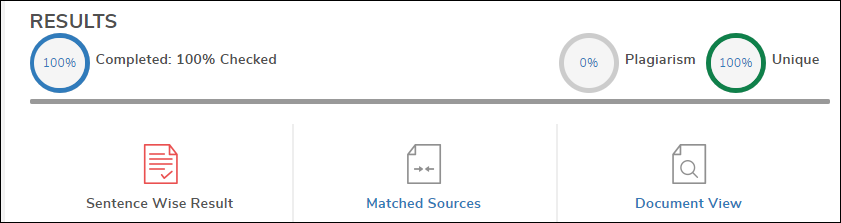
\includegraphics[width=0.5\textwidth]{figures/chapter6/1164074/3}}
	\caption{Hasil Check Data Plagiarisme}
	\label{data3}
\end{figure}
\end{enumerate}

\section{Yusniar Nur Syarif Sidiq / 1164089}
\subsection{Pemahaman Teori}

\begin{enumerate}

\item Apa itu fungsi library matplotlib ?
	\subitem Library Matplotllib adalah library python dengan 2D yang dapat menghasilkan plot dengan kualitas yang cukup tinggi dalam berbagai format dan dapat digunakan di beberbagai macam platform. Fungsi dari Library Matplotlib ini yaitu membuat grafik dalam berbagai bentuk seperti grafik diagram batang, berbentuk garis, lingkaran, histogram, dan lain sebagainya.

\item Jelaskan langkah - langkah membuat sumbu X dan Y di matplotlib !

	\begin{itemize}
		\item Lakukan Import Library Matplotlib terlebih dahulu dengan source code seperti berikut,
			\lstinputlisting [firstline=1, lastline=2]{src/chapter6/1164089/1164089.py}
		\item Buatlah dua variabel yang dapat menampung nilai dengan source code seperti berikut,
			\lstinputlisting [firstline=6, lastline=7]{src/chapter6/1164089/1164089.py}
		\item Panggil variabel tersebut dengan fungsi plot seperti source code berikut ini,
			\lstinputlisting [firstline=9, lastline=9]{src/chapter6/1164089/1164089.py}
		\item Untuk menamilkan hasilnya gunakan show seperti source code berikut ini,
			\lstinputlisting [firstline=11, lastline=11]{src/chapter6/1164089/1164089.py}
		\item Sehingga hasilnya dapat kita lihat di figure \ref{YNC6-1}
	\end{itemize}

	\begin{figure}[!htbp!]
		\centerline{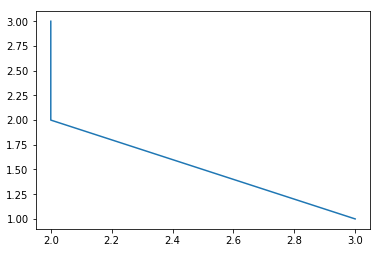
\includegraphics[width=0.5\textwidth]{figures/chapter6/1164089/YNC6-1.png}}
		\caption{Hasil Melakukan Plot Sumbu X dan Y.}
		\label{YNC6-1}
	\end{figure}

\item Jelaskan bagaimana perbedaan fungsi dan cara pakai untuk berbagai jesnis (bar, histogram, scatter, dll) jenis plot di matplotlib !

	\begin{itemize}

		\item Diagram Batang atau Bar Graphic dimana fungsi ini akan melakukan plot dan menampilkannya dengan bentuk diagram 			         batang, untuk membuat source codenya perhatikan dibawah dan hasilnya akan ditampilkan pada figure \ref{YNC6-1}.
		         \lstinputlisting [firstline=15, lastline=27]{src/chapter6/1164089/1164089.py}

			\begin{figure}[!htbp!]
				\centerline{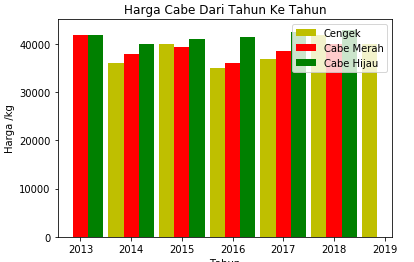
\includegraphics[width=0.5\textwidth]{figures/chapter6/1164089/YNC6-2.png}}
				\caption{Fungsi Bar.}
				\label{YNC6-2}
			\end{figure}

		\item Histogram, dimana pada fungsi ini akan melakukan plot penggabungan data yang telah dikelompokkan, untuk 				         membuatnya perhatikan source code dibawah dan hasilnya akan ditampilkan pada figure \ref{YNC6-3}.
		         \lstinputlisting [firstline=31, lastline=39]{src/chapter6/1164089/1164089.py}

			\begin{figure}[!htbp!]
				\centerline{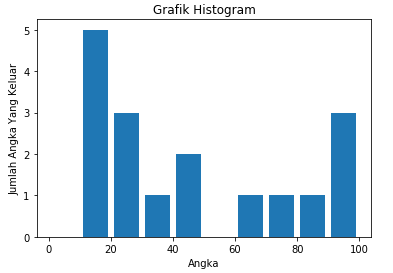
\includegraphics[width=0.5\textwidth]{figures/chapter6/1164089/YNC6-3.png}}
				\caption{Fungsi Histogram.}
				\label{YNC6-3}
			\end{figure}

		\item Scatter Plot, dimana fungsi ini akan melakukan plot berbentuk titik-titik yang masing-masing memiliki nilai variabel, 				         untuk membuatnya perhatikan source code dibawah dan hasilnya akan ditampilkan pada figure \ref{YNC-4}.
		        \lstinputlisting [firstline=43, lastline=56]{src/chapter6/1164089/1164089.py}

		        \begin{figure}[!htbp!]
				\centerline{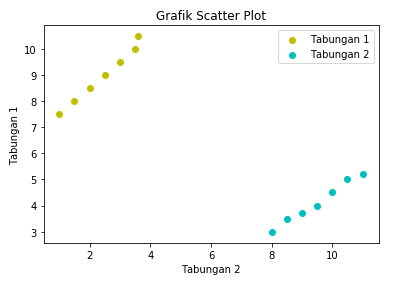
\includegraphics[width=0.5\textwidth]{figures/chapter6/1164089/YNC6-4.png}}
				\caption{Fungsi Scatter Plot.}
				\label{YNC6-4}
			\end{figure}

		\item Area Plot, dimana fungsi ini akan melakukan pelacakan terhadap perubahan antar dua kelompok atau lebih yang 				         terkait satu kategori secara keseluruhan, untuk membuatnya perhatikan source code dibawah dan hasilnya akan 				         ditampilkan pada figure \ref{YNC6-5}.
		        \lstinputlisting [firstline=60, lastline=79]{src/chapter6/1164089/1164089.py}

		         \begin{figure}[!htbp!]
				\centerline{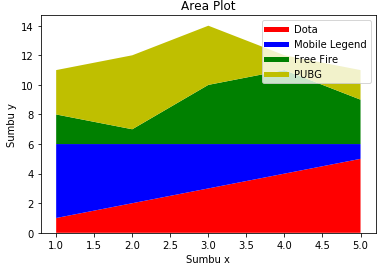
\includegraphics[width=0.5\textwidth]{figures/chapter6/1164089/YNC6-5.png}}
				\caption{Fungsi Area Plot.}
				\label{YNC6-5}
			\end{figure}

		\item Pie Plot, dimana pada fungsi ini akan digunakan dalam menunjukkan presentase yang mewakili setiap kategori, untuk 			         membuatnya perhatikan source code dibawah dan hasilnya akan ditampilkan pada figure \ref{YNC6-6}.
		         \lstinputlisting [firstline=83, lastline=104]{src/chapter6/1164089/1164089.py}

		         \begin{figure}[!htbp!]
				\centerline{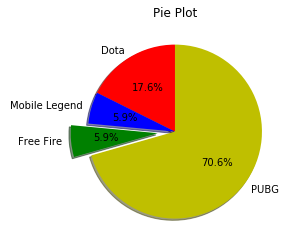
\includegraphics[width=0.5\textwidth]{figures/chapter6/1164089/YNC6-6.png}}
				\caption{Fungsi Pie Plot.}
				\label{YNC6-6}
			\end{figure}

		\item Line Graphic, dimana fungsi ini akan melakukan plot dengan bentuk line, untuk membuatnya perhatikan source code 			         dibawah dan hasilnya akan ditampilkan pada figure \ref{YNC6-7}.
		         \lstinputlisting [firstline=108, lastline=116]{src/chapter6/1164089/1164089.py}

		         \begin{figure}[!htbp!]
				\centerline{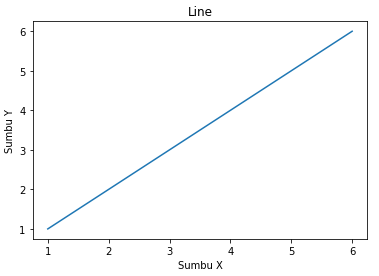
\includegraphics[width=0.5\textwidth]{figures/chapter6/1164089/YNC6-7.png}}
				\caption{Fungsi Line Graphic.}
				\label{YNC6-7}
			\end{figure}

	\end{itemize}

\item Jelaskan bagaimana cara menggunakan legend dan label serta kaitannya fungsi tersebut !
	
	\begin{itemize}

		\item Pertama kita akan membuat 4 variabel terlebih dahulu, perhatikan source code berikut,
		         \lstinputlisting [firstline=120, lastline=125]{src/chapter6/1164089/1164089.py}

		\item Dalam membuat fungsi legend kita akan mendefinisikan parameter label pada fungsi plot, dimana parameter label ini 			         akan digunakan untuk memberikan keterangan pada tiap line, perhatikan source code dibawah ini,
		         \lstinputlisting [firstline=126, lastline=127]{src/chapter6/1164089/1164089.py}

		\item Selanjutnya kita akan memberikan title dan nama pada setiap sumbu, gunakan source code seperti berikut,
		         \lstinputlisting [firstline=128, lastline=130]{src/chapter6/1164089/1164089.py}

		\item Panggil fungsi legend dan tampilkan di console gunakan source code berikut,
		         \lstinputlisting [firstline=131, lastline=133]{src/chapter6/1164089/1164089.py}

		\item Hasilnya dapat kita lihat pada figure \ref{YNC6-8}

	\end{itemize}

		\begin{figure}[!htbp!]
			\centerline{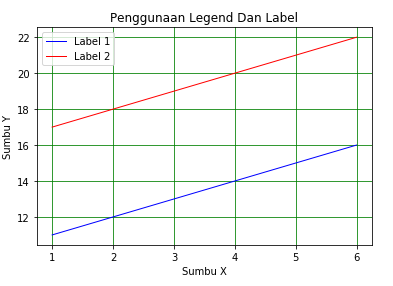
\includegraphics[width=0.5\textwidth]{figures/chapter6/1164089/YNC6-8.png}}
			\caption{Fungsi Legend Dan Label.}
			\label{YNC6-8}
		\end{figure}

\item Jelaskan apa fungsi dari subplot di matplotlib, dan bagaimana cara kerja dari fungsi subplot, sertakan ilustrasi dan gambar sendiri dan apa parameternya jika ingin menggambarkan plot dengan 9 subplot di dalamnya !
	\subitem Fungsi Subplot digunakan untuk membuat plot di dalam satu gambar, dimana fungsi subplot memiliki parameter pertama akan menentukan kolomnya, dan pada parameter kedua akan menentukan jumlah barisnya, dan parameter ketiga akan menentukan index plotnya, untuk membuatnta perhatikan source code dibawah dan hasilnya akan ditampilkan pada figure \ref{YNC6-9}.
	\lstinputlisting [firstline=137, lastline=149]{src/chapter6/1164089/1164089.py}

		\begin{figure}[!htbp!]
			\centerline{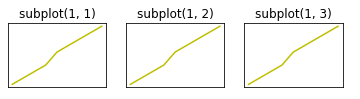
\includegraphics[width=0.5\textwidth]{figures/chapter6/1164089/YNC6-9.png}}
			\caption{Fungsi Subplot.}
			\label{YNC6-9}
		\end{figure}

\item Sebutkan semua parameter color yang bisa digunakan (contoh: m,c,r,k,...dkk) !
	\subitem Ada beberapa parameter warna yang dapat kita gunakan pada library matplotlib ini yaitu :
	\begin{itemize}
		\item r menunjukkan arti red
		\item b menunjukkan arti blue
		\item g menunjukkan arti green
		\item c menunjukkan arti cyan
		\item y menunjukkan arti yellow
		\item m menunjukkan arti magenta
		\item k menunjukkan arti black
		\item w menunjukkan arti white
	\end{itemize}

\item Jelaskan bagaimana cara kerja dari fungsi hist, sertakan ilustrasi dan gambar sendiri !
	\subitem Cara kerja dari fungsi hist atau biasa kita sebut dengan histogram, dimana akan melakukan eksekusi terhadap data yang telah dikelompokkan dan akan ditampilkan perhitungan jumlah data yang keluar, misalnya saya akan memprediksi jumlah angka yang akan keluar ada berapa, maka dibutuhkan lah source code seperti berikut,
	\lstinputlisting [firstline=31, lastline=39]{src/chapter6/1164089/1164089.py}
Hasil dari source code tersebut akan diperlihatkan pada figure \ref{YNC6-10}.

		\begin{figure}[!htbp!]
			\centerline{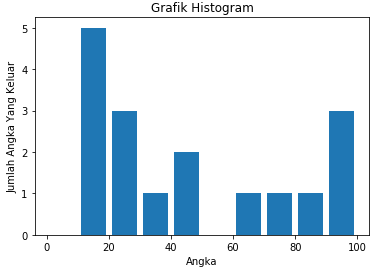
\includegraphics[width=0.5\textwidth]{figures/chapter6/1164089/YNC6-10.png}}
			\caption{Fungsi Subplot.}
			\label{YNC6-10}
		\end{figure}

\item Jelaskan lebih mendalam tentang parameter dari fungsi pie diantarannya labels, colors, startangle, shadow, explode, autopct !

	\begin{itemize}
		\item Labels digunakan untuk memberikan keterangan pada tiap presentase
		\item Colors digunakan untuk memberikan warna pada tiap presentase agar terlihat berbeda-beda
		\item Startangle digunakan untuk memutar plot dengan derajat yang telah ditentukan
		\item Shadow digunakan untuk memberikan efek bayangan pada plot
		\item Explode digunakan untuk memisahkan tiap potongan pie pada plot
		\item Autopct digunakan untuk menentukan jumlah angka dibelakang koma
	\end{itemize}

\end{enumerate}

\subsection{Keterampilan Pemrograman}
\begin{enumerate}

\item Buatlah Library Fungsi dengan nama NPM\_bar.py untuk plot dengan jumlah subplot adalah NPM mod 3 + 2 !
	\lstinputlisting [firstline=1, lastline=20]{src/chapter6/1164089/1164089_bar.py}
	\subitem Hasil dari source code tersebut akan menampilkan 4 biji bar, dikarenakan figure yang terlalu besar saya sceenshoot 				    seperti pada figure \ref{YNC6-11}.

	\begin{figure}[!htbp!]
		\centerline{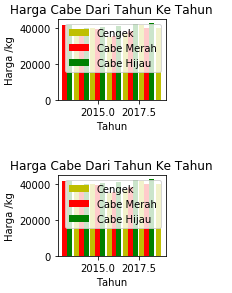
\includegraphics[width=0.5\textwidth]{figures/chapter6/1164089/YNC6-11.png}}
		\caption{Fungsi Bar Praktikum.}
		\label{YNC6-11}
	\end{figure}

\item Buatlah Library Fungsi dengan nama NPM\_scatter.py untuk plot dengan jumlah subplot NPM mod 3 + 2 !
	\lstinputlisting [firstline=1, lastline=22]{src/chapter6/1164089/1164089_scatter.py}
	\subitem Pada source code tersebut dapat dilihat pada figure \ref{YNC6-12}.

	\begin{figure}[!htbp!]
		\centerline{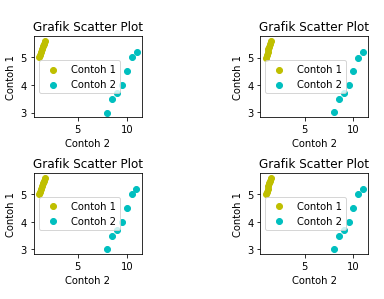
\includegraphics[width=0.5\textwidth]{figures/chapter6/1164089/YNC6-12.png}}
		\caption{Fungsi Scatter Praktikum.}
		\label{YNC6-12}
	\end{figure}

\item Buatlah Library Fungsi dengan nama NPM\_pie.py untuk plot dengan jumlah subplot NPM mod 3 + 2 !
	\lstinputlisting [firstline=1, lastline=22]{src/chapter6/1164089/1164089_pie.py}
	\subitem Pada source code tersebut dapat dilihat pada figure \ref{YNC6-13}.

	\begin{figure}[!htbp!]
		\centerline{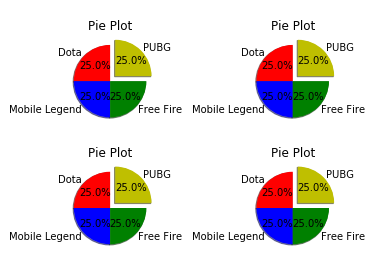
\includegraphics[width=0.5\textwidth]{figures/chapter6/1164089/YNC6-13.png}}
		\caption{Fungsi Pie Praktikum.}
		\label{YNC6-13}
	\end{figure}

\item Buatlah Library Fungsi dengan nama NPM\_plot.py untuk plot dengan jumlah subplot NPM mod 3 + 2 !
	\lstinputlisting [firstline=1, lastline=22]{src/chapter6/1164089/1164089_plot.py}
	\subitem Pada source code tersebut dapat dilihat pada figure \ref{YNC6-14}.

	\begin{figure}[!htbp!]
		\centerline{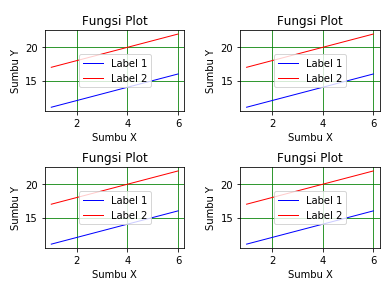
\includegraphics[width=0.5\textwidth]{figures/chapter6/1164089/YNC6-14.png}}
		\caption{Fungsi Plot Praktikum.}
		\label{YNC6-14}
	\end{figure}

\end{enumerate}

\subsection{Keterampilan Penanganan Error}

\begin{enumerate}

\item Error yang saya dapatkan terlihat pada figure \ref{YNC6-15} yang merupakan NameError dikarenakan variabel yang saya deklarasikan tidak sesuai, cara membenarkannya kita ganti variabel tersebut menjadi x dan y, dan untuk membuat fungsi try exceptnya dapat perhatikan source code berikut ini,

	\lstinputlisting [firstline=177, lastline=187]{src/chapter6/1164089/1164089.py}

	\begin{figure}[!htbp!]
		\centerline{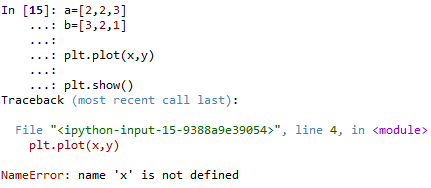
\includegraphics[width=0.5\textwidth]{figures/chapter6/1164089/YNC6-15.png}}
		\caption{Error Yang Di Dapat.}
		\label{YNC6-15}
	\end{figure}

\end{enumerate}

\section {Kevin Natanae Nainggolan 1174059}
	\subsection {TEORI}
	\begin {enumerate}
		\item  Apa itu fungsi library matplotlib
			\newline Library plotting 2 dimensi Python yang menciptakan gambar publikasi bermutu di dalam berbagai macam format hardcopy
		\item Jelaskan langkah-langkah membuat sumbu X dan Y di matplotlib
			\newline  Membuat sumbu x dan y pada matplotlib, kita bisa membuatnya menggunakan list untuk mempermudah penyimpanan nilai setiap sumbunya. Seperti kode di bawah
			\lstinputlisting [firstline=2, lastline=5]{src/chapter6/teori/1174059.py}
		\item Jelaskan bagaimana perbedaan fungsi dan cara pakai untuk berbagai jenis(bar,histogram,scatter,line dll) jenis plot di matplotlib
			\newline Untuk membedakan fungsi plot yang digunakan adalah dengan melihat bentuk grafik yang akan di tampilkan sesuai dengan perintah yang digunakan pada pemogramannya, dan untuk cara pengguna plot tersebut bisa dilihat sebagai berikut
			\lstinputlisting [firstline=2, lastline=2]{src/chapter6/teori/1174059.py}
				\begin {enumerate}
					\item bar 
					\newline Perhatikan kode dalam membentuk diagram bar seperti berikut
						\lstinputlisting [firstline=21, lastline=29]{src/chapter6/teori/1174059.py}
					\item histogram
					\newline Dalam penggunaanya plot bar x dan y dapat diatur dengan angka koma
						\lstinputlisting [firstline=35, lastline=41]{src/chapter6/teori/1174059.py}
					\item scatter
					\newline Diagram yang penampilannya dengan titik titik sebagai penandanya
						\lstinputlisting [firstline=46, lastline=56]{src/chapter6/teori/1174059.py}
					\item line
					\newline Perhatikan kode dalam membentuk diagram line seperti berikut
						\lstinputlisting [firstline=13, lastline=16]{src/chapter6/teori/1174059.py}
					\item stack plot
					\newline Penggunaan stack plot ini seperti diagram line, dengan warna yang mengisinua, serta antar line itu bisa berdekatan. Berikut Contoh penggunaannya
						\lstinputlisting [firstline=61, lastline=83]{src/chapter6/teori/1174059.py}
				\end {enumerate}
		\item Jelaskan bagaimana cara menggunakan legend dan label serta kaitannya dengan fungsi tersebut
		\newline Penggunaan legend untuk memudahkan dalam membaca grafik. Dalam penggunaan lagend dan label perhatikan code berikut
			\lstinputlisting [firstline=55, lastline=55]{src/chapter6/teori/1174059.py}
		\item Jelaskan apa fungsi dari subplot di matplotlib, dan bagaimana cara kerja dari fungsi subplot, sertakan ilustrasi dan gambar sendiri dan apa parameternya jika ingin menggambar plot dengan 9 subplot di dalamnya
		\newline fungsi dari subplot dari matplotlib untuk bisa membuat lebih dari 1 grafik dalam sebuah program. Untuk parameternya sendiri kami menggunakan t1 dan t2. Cara kerjanya sendiri bisa d cek sebagai berikut
			\lstinputlisting [firstline=87, lastline=112]{src/chapter6/teori/1174059.py}
		\item Sebutkan semua parameter color yang bisa digunakan (contoh: m,c,r,k,... dkk)
			\begin {itemize}
				\item R untuk warna Red atau Merah
				\item G untuk warna Green atau Hijau
				\item B untuk warna Blue atau Biru
				\item C untuk warna Cyan atau Biru Muda
				\item M untuk warna Mangenta atau Merah Tua
				\item Y untuk warna Yellow Atau Kuning
				\item K untuk warna blacK atau Hitam
			\end {itemize}
		\item Jelaskan bagaimana cara kerja dari fungsi hist, sertakan ilustrasi dan gambar sendiri
		\newline  Fungsi hist digunakan untuk menjumlahkan beberapa data yang memenuhi kriteria pramater yang kita tentukan, seprti contoh kode dibawah
			\lstinputlisting [firstline=116, lastline=121]{src/chapter6/teori/1174059.py}
		\item Jelaskan lebih mendalam tentang parameter dari fungsi pie diantaranya labels, colors, startangle, shadow, explode, autopct
			\newline  
			\begin{itemize}
	\item labels : Isi dengan tipe data list dan tidak wajib untuk digunakan. Fungsi parameter labels untuk memberi label pada setiap pecahan data yang ada pada grafik pie yang ditampilkan.
	\item colors : Tipe data array atau sejenis dan tidak wajib untuk digunakan. Fungsi parameter colors untuk mengganti warna pada setiap pecahan yang ada. Jika tidak digunakan atau ditentukan, maka warna yang akan dipakai adalah warna yang aktif atau standar.
	\item startangle : Tipe data pecahan atau float, tidak wajib untuk digunakan. Fungsi parameter startangle adalah fungsi untuk memutar grafik agar berubah posisi dengan acuan yaitu angle awalan dari grafik pie.
	\item shadow : Bertipe data boolean dan tidak wajib digunakan. Fungsi parameter shadow digunakan untuk membuat bayangan pada bawah grafik pie yang ditampilkan. 
	\item explode : Bertipe data array atau sejenis dan tidak wajib digunakan. Fungsi parameter explode adalah menentukan radius untuk mengimbangi setiap pecahan pada grafik pie. Jika radius lebih dari 0 maka pecahan akan mulai menjauh dari pusat dan terlihat seperti keluar dari grafik lingkaran tersebut.
	\item autopct : Bertipe data string atau fungsi dan tidak wajib digunakan. Fungsi parameter autopct adalah memberi label pada irisan dengan labelnya berupa fungsi atau string. 
			\end{itemize}
	\end {enumerate}
	
		\subsection {PRAKTEK}
		\begin {enumerate}
			\item Buatlah librari fungsi (file terpisah/library dengan nama NPM bar.py) untuk plot dengan jumlah subplot adalah NPM mod 3 + 2
				\lstinputlisting [firstline=8, lastline=27]{src/chapter6/praktek/1174059/chap6_1174059_bar.py}
			\item Buatlah librari fungsi (file terpisah/library dengan nama NPM scatter.py) untuk plot dengan jumlah subplot NPM mod 3 + 2
				\lstinputlisting [firstline=8, lastline=38]{src/chapter6/praktek/1174059/chap6_1174059_pie.py}
			\item Buatlah librari fungsi (file terpisah/library dengan nama NPM pie.py) untuk plot dengan jumlah subplot NPM mod 3 + 2
				\lstinputlisting [firstline=8, lastline=27]{src/chapter6/praktek/1174059/chap6_1174059_scater.py}
			\item Buatlah librari fungsi (file terpisah/library dengan nama NPM plot.py) untuk plot dengan jumlah subplot NPM mod 3 + 2
				\lstinputlisting [firstline=8, lastline=27]{src/chapter6/praktek/1174059/chap6_1174059_plot.py}
		\end {enumerate}
		
	\subsection {PENANGANAN EROR}
		Tuliskan peringatan error yang didapat dari mengerjakan praktek ketiga ini, dan jelaskan cara penanganan error tersebut. dan Buatlah satu fungsi yang menggunakan gunakan try except untuk menanggulangi error tersebut
		\lstinputlisting [firstline=8, lastline=30]{src/chapter6/praktek/1174059/chap6_1174059_penanganan.py}